\chapter{Navigation}

For the navigation part it has been used the \Acrshort{nav2} package, as described in \autoref{cha:techstack}. As said, the only thing necessary to do is passing a YAML config file to \code{navigation\_bringup.py} in order to start the desired nodes with the desired parameters set. It is easier said than done. (?)

\section{\Acrshort{nav2} nodes introduction}

This is a brief description of the nodes responsible for the navigation, in order to have a better idea of the workflow, mostly thanks to \Acrshort{nav2} README files of the GitHub repository \cite{nav2github}.

\subsection*{Lifecycle Manager}

Lifecycle Manager harnesses the {\it managed nodes}\footnote{A managed life cycle for nodes allows greater control over the state of ROS system. [...] a managed node presents a known interface, executes according to a known life cycle state machine, and otherwise can be considered a black box \cite{lifecycle}.} \Acrshort{ros}2 concept to navigation stack: in such a manner, before nodes start executing, it checks if all of them were launched correctly and are ready, to avoid unexpected behavior. 

\begin{figure}[h]
    \centering
    \begin{minipage}[h]{0.45\textwidth}
        \centering
        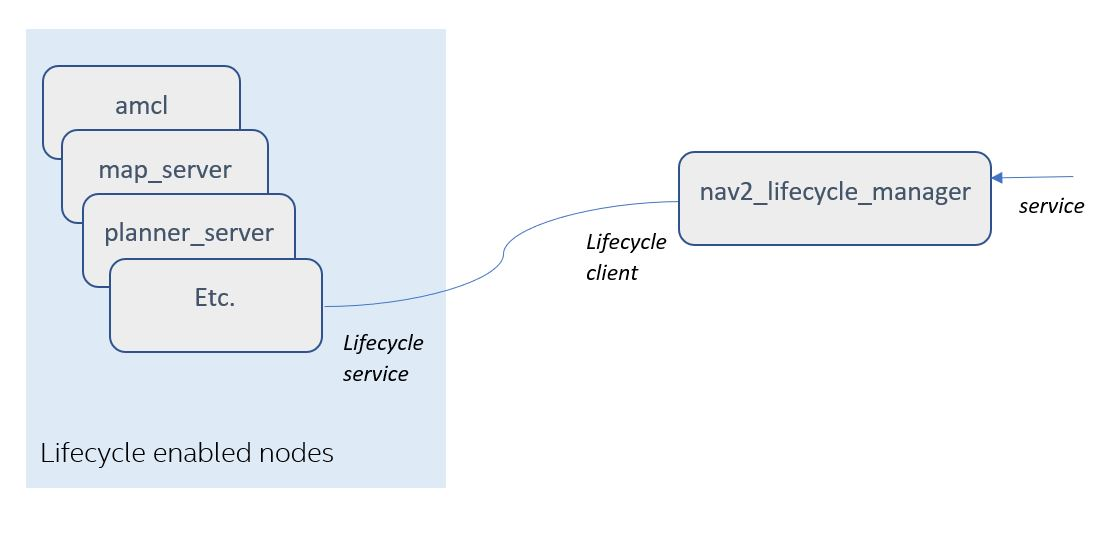
\includegraphics[width=\textwidth]{images/diagram_lifecycle_manager}
        \caption{Interaction between managed nodes and the lifecycle manager}
    \end{minipage}
    \hfill  
    \begin{minipage}[h]{0.45\textwidth}
        \centering
        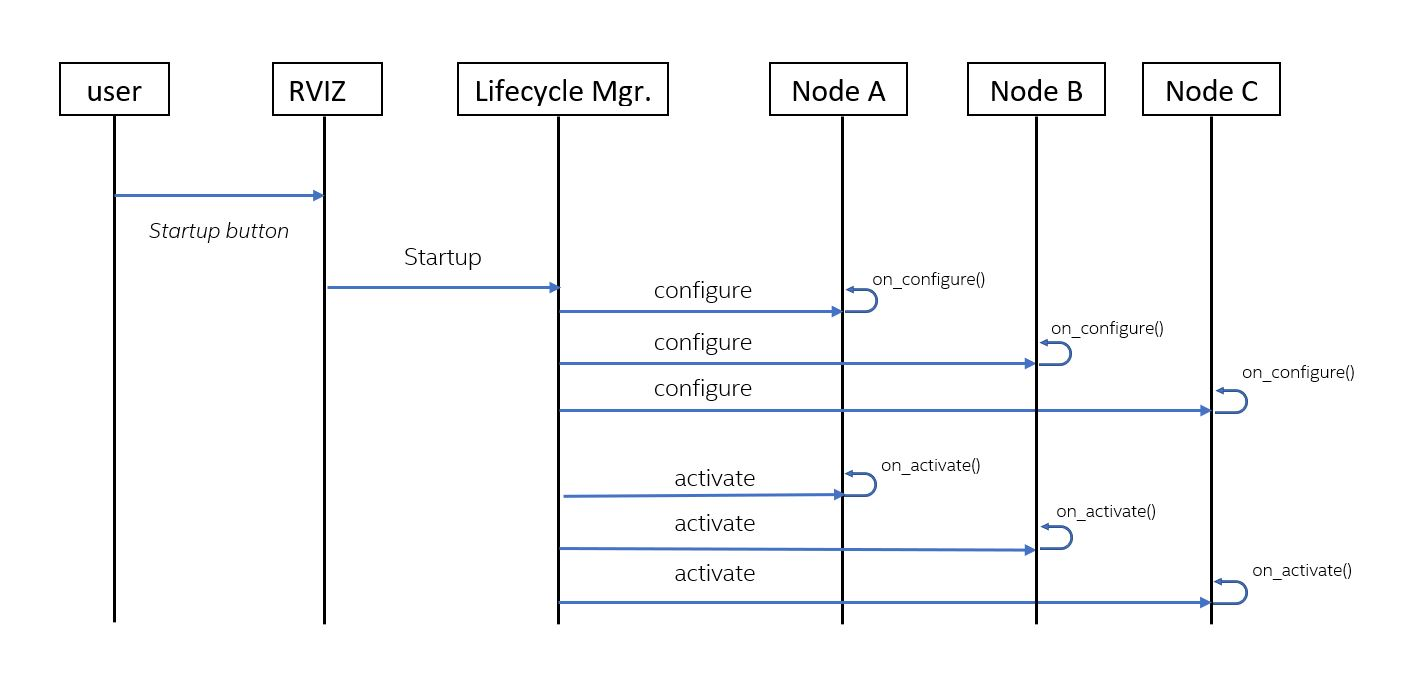
\includegraphics[width=\textwidth]{images/uml_lifecycle_manager}
        \caption{Sequence of service calls when startup is requested}
    \end{minipage}
\end{figure}

\subsection*{Planner server}

It implements behavior trees to compute path to pose, to which is possible to attach plugins.

\subsection*{Controller server}

It generates command velocities for the robot, using computed path from planner server.

\subsection*{Map Server}

This package is used to provide map functionalities to \Acrshort{ros}. Basically, it gives you the possibility to load a map from a file or save it after \Acrfull{slam} has been run.

\subsection*{Recoveries server}

It is responsible for executing simple controlled robot movements, like backing up, rotating and stopping when recovery is needed.

\subsection*{Waypoint Follower (?)} 

In \Acrshort{rviz} is also implemented the possibility to navigate the robot between specified waypoints: after they have been set, a feedback is periodically returned, and when completed returns the missed waypoints. This functionality has not been used in the following chapter (cite (?)), but could be useful for other testing purposes.

\subsection*{\Acrfull{amcl}}

\Acrshort{amcl} is used to localize the robot on a known map using a 2D laser scanner probabilistically.
. Firstly, once the map is loaded, the initial robot pose must be set\footnote{\Acrshort{rviz} lets you set the initial robot pose graphically.}: what is going on under the hood is publishing a \code{map} $\rightarrow$ \code{odom} transformation so that the \code{odom} $\rightarrow$ \code{base\_link} one leads to the real position of the robot.

\subsection*{\Acrfull{btnav}}

This one makes use of behavior trees to define the actions to be performed when the robot is in a certain state: for example, when no problem has met, it will continue to navigate and reach the current goal, but when it hits something, the behavior tree will execute the recovery action.

\begin{figure}[h]
    \centering
    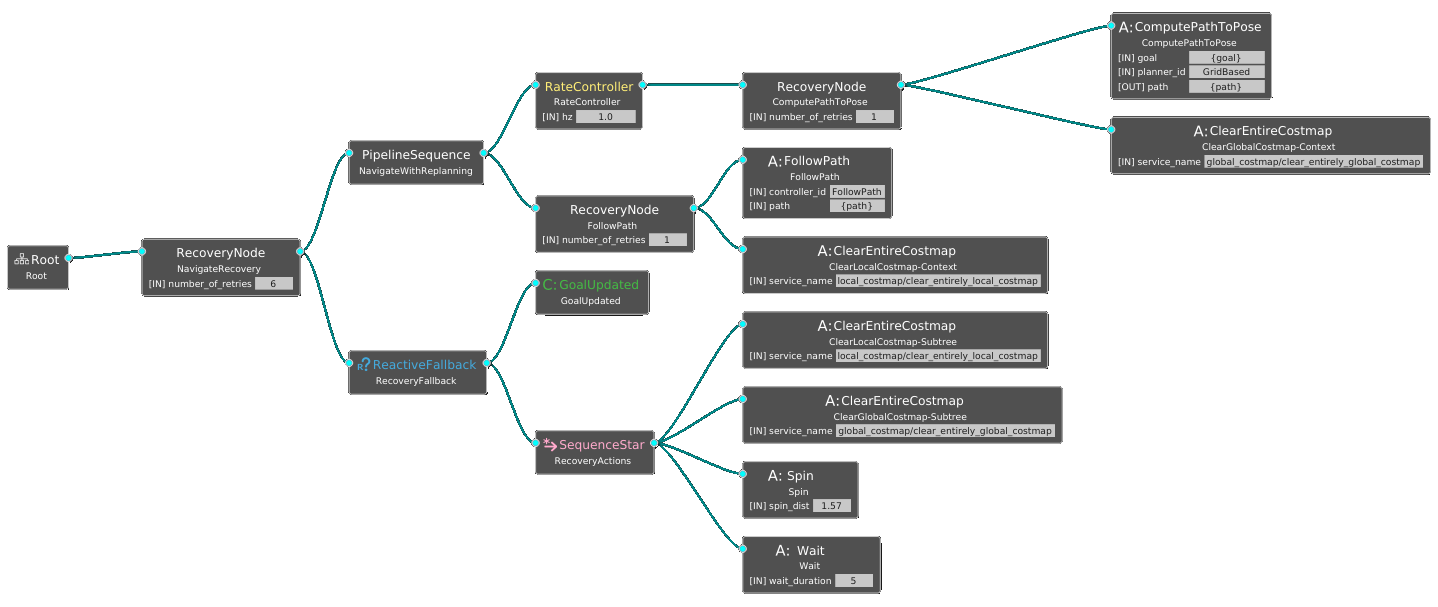
\includegraphics[width=\textwidth]{images/bt-alpha.png}
    \caption{Currently used behavior tree. Thanks to Groot, it is possible to visualize the robot behavior, also in real-time \cite{groot}.}
\end{figure}

\subsection*{\Acrfull{slam}}

It is a collection of techniques used to localize and map the environment simultaneously, using 2D laser scans. Once the map is completely built, it is possible to save it to a file, and pass it to the map server \cite{slam}.

\section{\code{g\_robot} package integration}

Everything required to navigate through the environment is provided by \code{g\_robot} package. The complete structure is shown in the following figure.

\begin{wrapfigure}{l}{0.3\textwidth}
  \captionsetup{singlelinecheck = false, format= hang, justification=raggedright, font=footnotesize, labelsep=space}
  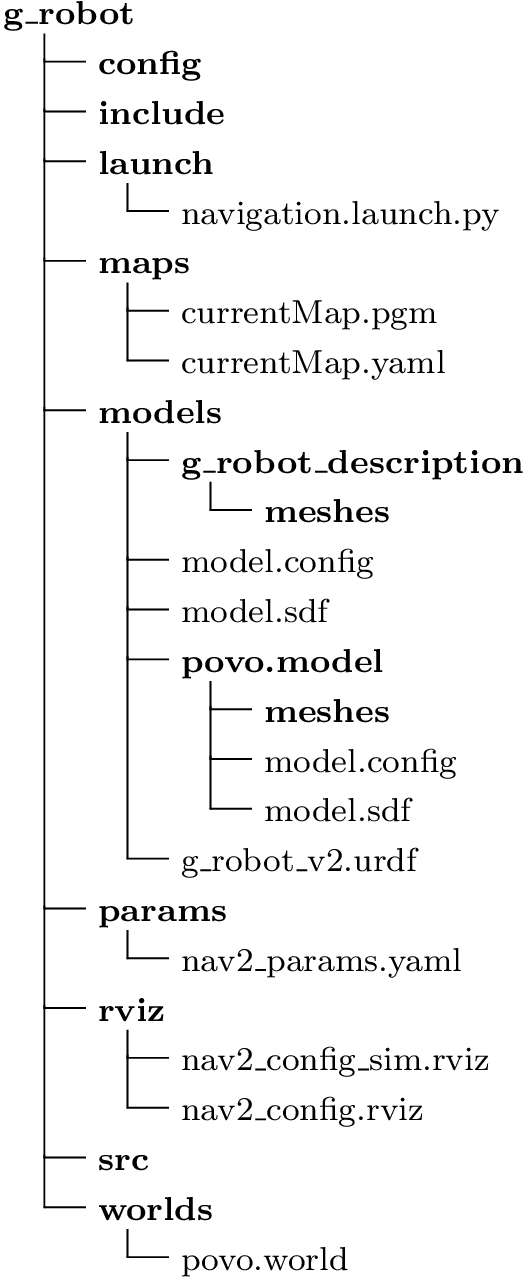
\includegraphics[width=0.3\textwidth]{images/g-robot}
  \caption{Folder structure of g\_robot package}
\end{wrapfigure}

% TODO: sistemare folder structure (togliere v2 da urdf e aggiugnere "..." se una cartella contiene altri file; sistemare altezza lidar? 0.45 invece di 0.41 come su shelfino?)